\documentclass[11pt]{article}

\usepackage[margin=1in, a4paper]{geometry}

\usepackage[utf8]{inputenc}

\usepackage{setspace}  % set spacing

\setstretch{1.25}  %stretch line space to multiple x

\usepackage[dvipsnames,table, xcdraw]{xcolor}
% If you use beamer only pass "xcolor=table" option, i.e. \documentclass[xcolor=table]{beamer}

\usepackage{shadowtext}

\usepackage{indentfirst} % indent the first paragraph of each section

\usepackage{float} %determine the position of figures in the document

\usepackage{tabularx} % extra features for tabular environment

\usepackage{amsmath, amsfonts, amssymb}  % improve math presentation
\allowdisplaybreaks

\usepackage{blkarray, bigstrut}

\usepackage{makecell}

\usepackage{mathtools}
\DeclarePairedDelimiter\ceil{\lceil}{\rceil}
\DeclarePairedDelimiter\floor{\lfloor}{\rfloor}



%++++++++++++++++++++++++++++++++++++++++++++++++++++++++++++++++

\usepackage{graphicx} % takes care of graphic including machinery

\graphicspath{ {../../logos/} }

%++++++++++++++++++++++++++++++++++++++++++++++++++++++++++++++++



\usepackage{caption}

\usepackage{subcaption}

\usepackage{tikz}
\usetikzlibrary{shapes}

\usepackage{lipsum,lmodern}

\usepackage[most]{tcolorbox}

\usetikzlibrary{trees}  %add binary trees

\usetikzlibrary {positioning}

\usepackage[final]{hyperref} % adds hyper links inside the generated pdf file

\hypersetup{
	colorlinks=true,       % false: boxed links; true: colored links
	linkcolor=blue,        % color of internal links
	citecolor=blue,        % color of links to bibliography
	filecolor=magenta,     % color of file links
	urlcolor=blue         
}

\usepackage{blindtext}

\usepackage{dirtytalk} %quotation marks


%********************************

%Bibliography

\usepackage[backend=biber,  style=alphabetic,  sorting=ynt]{biblatex}

\addbibresource{../../Mybib.bib}


%********************************


\usepackage{fancyhdr}

\pagestyle{fancy}

\fancyhf{}

\lhead{\footnotesize {Math notes: Gamma Distribution} }
\rhead{\footnotesize { } }
\cfoot{- \thepage \ -}

\title{\vspace{-90pt} 


%**************************************************

% Title Part
\textbf  {Peer-graded Assignment} }
\author{Cui, Xiaolong(Larry)}
\date{\today}


%*************************************************

\begin{document}

%\maketitle

\thispagestyle{plain}

%*************************************************

\begin{figure}[H] %[!tbp]
  \begin{subfigure}{0.3\textwidth}
    
\includegraphics[width=\textwidth]{uol}
    %\caption{Flower one.}
    %\label{fig:f1}
  \end{subfigure}
  \hfill
  \begin{subfigure}{0.3\textwidth}
    \includegraphics[width=\textwidth]{goldsmiths}
    %\caption{Flower two.}
    %\label{fig:f2}
  \end{subfigure}
  %\caption{My flowers.}
\end{figure}

%****************************************************

\begin{flushright}
\footnotesize {Oct. 5\textsuperscript{th} 2021}
\end{flushright}

\begin{center}
\textbf{The Gamma Distribution} \\
\footnotesize {Study Notes $ | $ Written by Larry Cui}
\end{center}

%***************************************************

%\begin{abstract}
%\end{abstract}


%***************************************************

\setcounter{figure}{0}

\vspace{10pt}


\section{\normalsize Prologue: waiting time variable}

Under a Poisson distribution $\displaystyle p_X (k) = \frac{e^{-\lambda y} (\lambda y)^k}{k!}$,  if we want to know the waiting time distribution of the next occurrence,  we would differentiate the cdf of all occurrences probability during the certain period of $y$:
\[
F_Y (y) = [1-P(Y=0)]= 1- e^{-\lambda y} \qquad {\color{RoyalBlue} \Rightarrow} \qquad f_Y (y) = \frac{d}{dy} F_Y(y) = \lambda e^{-\lambda y},  \quad y>0
\]

A little modification of this idea can bring it to a broader application: the waiting time distribution for the $r$th event occurrence.  

\begin{tcolorbox}[
	enhanced, 
	width=\textwidth, 
	%center upper,
	fontupper=\normalsize,% \bfseries,
	drop fuzzy shadow southwest,
	boxrule=0.4pt,
	sharp corners,
	colframe=yellow!80!black,
	colback=yellow!10]
	
\textbf{\color{RoyalBlue} lemma} \quad Suppose that Poisson events are occurring at the constant rate of $\lambda$ per unit time.  Waiting time $Y$ for the $r$th event has a pdf
\[ 
f_Y(y) = \frac{\lambda ^r}{(r-1)!} y^{r-1} e^{-\lambda y}, \quad y>0
\]

\end{tcolorbox}


\textbf{Proof:} To construct this formula, first of all,  we know that for $r$th event happening exactly on time point $y$,  $(r-1)$ events must happen first within $0 \backsim y$ period.  
\begin{equation}
\sum _{k=0} ^{r-1} e^{-\lambda y} \frac{(\lambda y)^k}{k!}
\end{equation}
\begin{equation}
F_Y (y) = 1- \sum _{k=0} ^{r-1} e^{-\lambda y} \frac{(\lambda y)^k}{k!}
\end{equation}

Eq. (1) is the probability of $(r-1)$ events happening within $y$ time period,  and Eq.  (2) is apparently the probability of $r$th and more events happening during the same period.  Differentiating $F_Y(y)$,  the meaning of which is to find the changing rate of $F$,  gives us the pdf of the $r$th event happening on time point $y$.  Someone may argue \say {why $r$th event?} After all, $F_Y(Y)$ is the cdf for $r$th and more events.  Well, $r$th event is the closest to happen,  and for $(r+1)$th and above,  we will have updated pdf for them.     

By differentiating:
\[
\begin{aligned}
f_Y(y) = F' _Y (y) 
	&= \frac{d}{dy} \left[ 1- \sum _{k=0} ^{r-1} e^{-\lambda y} \frac{(\lambda y)^k}{k!} \right ] \\
	&= \sum _{k=0} ^{r-1} \lambda e^{-\lambda y} \frac{(\lambda y)^k}{k!} - \sum _{k=1} ^{r-1} \lambda e^{-\lambda y} \frac{(\lambda y)^{k-1} }{(k-1)!}  & \quad & \color{RoyalBlue}  \text{\footnotesize Remark: } \left[ \frac{(\lambda y)^0}{0!} \right]' = 0\\
	&= \sum _{k=0} ^{r-1} \lambda e^{-\lambda y} \frac{(\lambda y)^k}{k!}  - \sum _{k=0} ^{r-2} \lambda e^{-\lambda y} \frac{(\lambda y)^k}{k!} \\
	&= \frac{\lambda ^r}{(r-1)!} y^{r-1} e^{-\lambda y}
\end{aligned}
\]



\section{\normalsize Gamma Function}


\begin{tcolorbox}[
	enhanced, 
	width=\textwidth, 
	%center upper,
	fontupper=\normalsize,% \bfseries,
	drop fuzzy shadow southwest,
	boxrule=0.4pt,
	sharp corners,
	colframe=yellow!80!black,
	colback=yellow!10]
	
\textbf{\color{RoyalBlue} Definition}  
\[ 
\Gamma (r) = \int _0 ^\infty y^{r-1} e^{-y} \, dy
\]

\end{tcolorbox}

Although we derive this function from the analysis of waiting time for $r$th event,  for the function itself,  $r$ is not necessarily to be any integers,  but real number.  We also have some interesting features for this gamma function:
\begin{itemize}
\item $\Gamma (1) = 1$ \\
proof: $\displaystyle \Gamma (1) = \int _0 ^\infty y^{1-1}e^{-y} \, dy = \int _0 ^  \infty e^{-y} \, dy = 1 $
\item $ \Gamma (r) = (r-1) \Gamma(r-1) $ \\
proof:  $\displaystyle \int _0 ^\infty y^{r-1} e^{-y} \, dy = -y^{r-1} e^{-y} \bigg | ^\infty _0  + \int _0 ^\infty (r-1) y^{r-2} e^{-y} \, dy = (r-1) \int _0 ^\infty y^{r-2} e^{-y} \, dy   $
\item if $r$ is an integer, then $\Gamma (r) = (r-1)!$ \\
proof: this is the result of direct application of the above two features.
\end{itemize}



\section{\normalsize Gamma pdf}


\begin{tcolorbox}[
	enhanced, 
	width=\textwidth, 
	%center upper,
	fontupper=\normalsize,% \bfseries,
	drop fuzzy shadow southwest,
	boxrule=0.4pt,
	sharp corners,
	colframe=yellow!80!black,
	colback=yellow!10]
	
\textbf{\color{RoyalBlue} Definition}  \quad a random variable $Y$ is said to have the gamma pdf with paramaters $r$ and $\lambda$ if
\[ 
f_Y(y) =\underbrace{ \frac{\lambda ^r}{\Gamma (r)} }_{\text {constant} } y^{r-1} e^{-\lambda y},  \quad y \geqslant 0
\]

\end{tcolorbox}


\textbf{Proof:} $f_Y(y)$ is always positive,  so the rest is to prove the sum adds up to 1.   If we let $y' = \lambda y,  dy' = \lambda \, dy$, the right part of the above equation
\[
\frac{1}{\Gamma(r)} \int _0 ^\infty \lambda ^r y^{r-1} e^{-\lambda y} \, dy
	= \frac{1}{\Gamma(r)}  \int _0 ^\infty {y'}^{(r-1)} e^{-y'} \, dy' 
	= \frac{1}{\Gamma(r)} \cdot  \Gamma(r)
	= 1
\]

The expected value and variance of Gamma pdf:
\[
\begin{aligned}
E(X)
	&= \frac{1}{\Gamma(r)} \int _0 ^\infty  y \cdot \lambda ^r y^{r-1} e^{-\lambda y} \, dy \\
	&= \frac{1}{\Gamma(r)} \frac{1}{\lambda} \int _0 ^\infty  u^r e^{-u} \, du && \color{RoyalBlue}  \text{\footnotesize Remark: } u = \lambda y, du = \lambda \,dy \\
	&= \frac{1}{\Gamma(r)} \frac{1}{\lambda} \cdot \Gamma(r+1) \\
	&= \frac{r}{\lambda} && \color{RoyalBlue}  \text{\footnotesize Remark: } \Gamma(r+1)= r \Gamma(r) \\
\end{aligned}
\]

\[
\begin{aligned}
Var(X)
	= E(X^2) - E(X)^2 
	&=\frac{1}{\Gamma(r)} \int _0 ^\infty  y^2 \cdot \lambda ^r y^{r-1} e^{-\lambda y} \, dy  - \frac{r^2}{\lambda ^2} \\
	&= \frac{1}{\Gamma(r)} \frac{1}{\lambda ^2} \int _0 ^\infty  u^{r+1} e^{-u} \, du  - \frac{r^2}{\lambda ^2} && \color{RoyalBlue}  \text{\footnotesize Remark: } u = \lambda y, du = \lambda \,dy \\
	&= \frac{1}{\Gamma(r)} \frac{1}{\lambda ^2} \cdot \Gamma(r+2) - \frac{r^2}{\lambda ^2} \\
	&= \frac{r}{\lambda ^2} && \color{RoyalBlue}  \text{\footnotesize Remark: } \Gamma(r+2)= (r+1)r \Gamma(r) \\
\end{aligned}
\]



\section{\normalsize Additive Property and \textit{mgf} }

The additive property of a variable means the sum of two or more independent variables \say {reproduce} the similar pdf.   Usually we see binomial,  Poisson or normal variables behave this way,  because in essence they all have \say {normal like} pdf.   Most other variables,  however,  don't have such property,  due to the central limit theorem.  


\begin{figure}[H] %[!tbp]
\centering
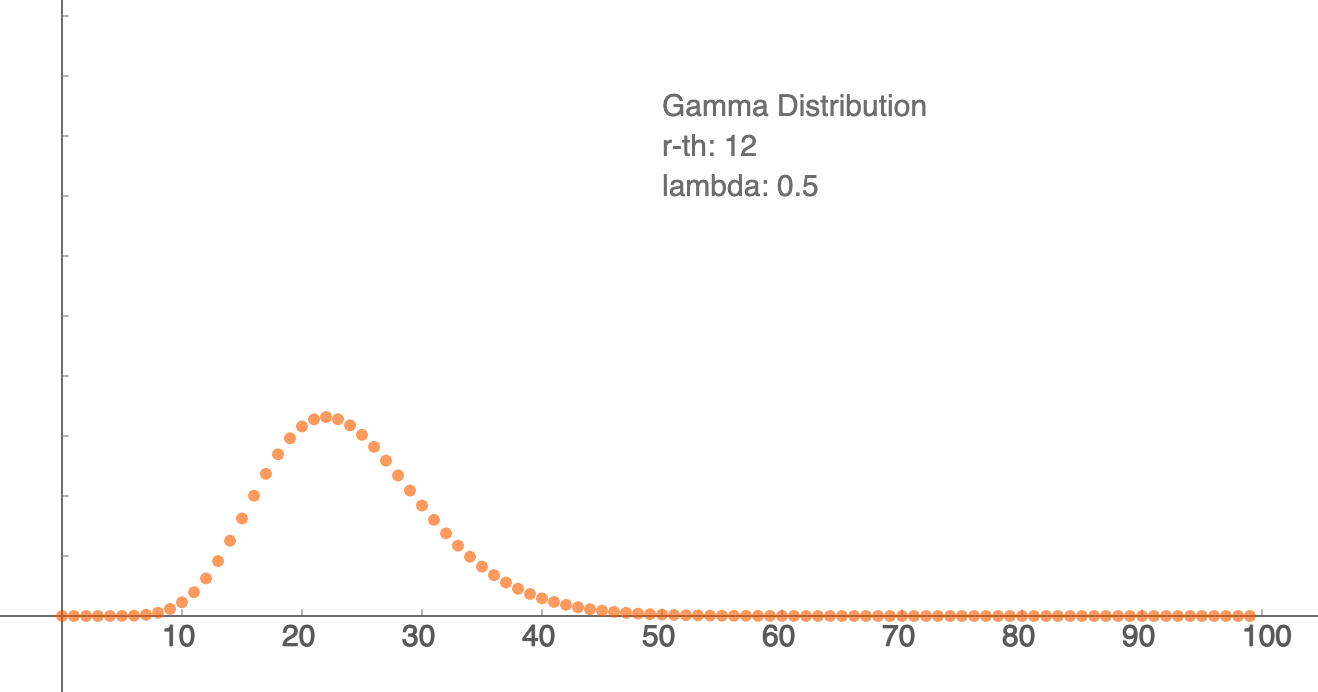
\includegraphics[width=0.7\textwidth]{gamma}
\caption{Gamma Distribution \textit{pdf} }
\label{fig:f1}
\end{figure}


\begin{tcolorbox}[
	enhanced, 
	width=\textwidth, 
	%center upper,
	fontupper=\normalsize,% \bfseries,
	drop fuzzy shadow southwest,
	boxrule=0.4pt,
	sharp corners,
	colframe=yellow!80!black,
	colback=yellow!10]
	
\textbf{\color{RoyalBlue} Additive Property of Gamma pdf}  

\qquad Suppose two independent variables $U$ has the gamma pdf with parameters $r$ and $\lambda$,  $V$ with $s$ and the same $\lambda$.  Then $U+V$ has a gamma pdf with parameters $r+s$ and $\lambda$. 

\end{tcolorbox}



\textbf{Proof}(direct, weak version):  Let $t= u + v$,  then pdf of $t$ is
\[
\begin{aligned}
f_{U+V} (t) 
	&= \int _0 ^t f_U(u) f_V(t-u) \, du && \color{RoyalBlue}  \text{\footnotesize Remark: both $u,v \geqslant 0 $,  so the scope of $u$ is $(0, t)$} \\ 
	&= \frac{\lambda^{r+s} } {\Gamma(r) \Gamma(s)} \int _0 ^t u^{r-1} e^{-\lambda u} (t-u)^{s-1} e^{-\lambda (t-u)} \, du \\
	&=  \frac{\lambda^{r+s} e^{-\lambda t} } {\Gamma(r) \Gamma(s)} \int _0 ^t u^{r-1} (t-u)^{s-1}  \, du \\
	&=  \frac{\lambda^{r+s} e^{-\lambda t} t^{r+s-1} } {\Gamma(r) \Gamma(s)} \int _0 ^1 x^{r-1} (1-x)^{s-1}  \, dx && \color{RoyalBlue}  \text{\footnotesize Let $x=u/t,  x \in (0, 1)$ } \\
\end{aligned}
\]
we can tell from the above formula that $\displaystyle e^{-\lambda t} t^{r+s-1} $ is the only changing part of the function and matches a gamma pdf with $r=r+s$ and $y=t$,  the rest is constant.  

Strong version: another way to prove the additive property is by mgf.  First of all, we find the $M_Y(t)$ of a gamma pdf
\[
\begin{aligned}
M_Y (t) 
	&= \int _0 ^\infty e^{ty} f_Y(y) \, dy \\ 
	&=  \frac{1}{\Gamma(r)} \int _0 ^\infty  e^{ty} \cdot \lambda ^r y^{r-1} e^{-\lambda y} \, dy \\
	&= \frac{\lambda ^r}{(\lambda - t) ^r} \cdot \left[ \frac{1}{\Gamma(r)} \int _0 ^\infty  (\lambda - t) ^r y^{r-1} e^{-(\lambda - t) y} \, dy \right] \\
	&= \left(1- \frac{t}{\lambda} \right) ^{-r}  \qquad  \color{RoyalBlue}  \text{\footnotesize in brackets is the integral of a gamma pdf with $\lambda = \lambda - t$ }\\
\end{aligned}
\]
Then we have
\[
M_U(t) = \left(1- \frac{t}{\lambda} \right) ^{-r} \quad \text {and} \quad M_V(t) = \left(1- \frac{t}{\lambda} \right) ^{-s}
\]
and
\[
M_{U+V} (t) = M_U(t) \cdot M_V(t) = \left(1- \frac{t}{\lambda} \right) ^{-(r+s)} 
\]

From this mgf,  we conclude the pdf of new variable $U+V$ has gamma pdf with $r=r+s$ and $\lambda$.
 








%++++++++++++++++++++++++++++++++++++++++

\clearpage

\printbibliography [title={Reference}]


%***********************************

\end{document}
